\documentclass[11pt, twocolumn]{article}


% \IEEEoverridecommandlockouts               % This command is only needed if
%                                            % you want to use the \thanks command

% \overrideIEEEmargins                     % Needed to meet printer requirements.

\usepackage[style=ieee]{biblatex}
\usepackage{amsmath}
\usepackage{graphicx}
\usepackage{fullpage}
\usepackage{subcaption}
\usepackage{url}
\usepackage{csquotes}
\usepackage[american]{babel}
\usepackage{comment}
\usepackage{amsthm}

\newtheorem{theorem}{Theorem}
\newtheorem{lemma}[theorem]{Lemma}

% \DeclareMathOperator{\atantwo}{atan2}

% \DeclareMathOperator{\arctantwo}{arctan2}

%\setlength{\belowcaptionskip}{-6pt}
\setlength{\textfloatsep}{8pt}

\newcommand{\parallelsum}{\mathbin{\!/\mkern-5mu/\!}}


\DeclareMathOperator{\atantwo}{atan2}

\DeclareMathOperator{\arctantwo}{arctan2}

\addbibresource{abrv.bib}
\addbibresource{refs-chains.bib}
\addbibresource{djbref.bib}
\addbibresource{swarm.bib}
\addbibresource{peg-in-hole.bib}


\title{The best peg and socket joint}
\author{Zhibin Zou \and Weifu Wang}
\date{}

\newcommand{\bo}{\mathbf o}
\newcommand{\bq}{\mathbf q}
\newcommand{\bp}{\mathbf p}
\newcommand{\bd}{\mathbf d}
\newcommand{\bn}{\mathbf n}
\newcommand{\bc}{\mathbf c}

\begin{document}
\maketitle

\begin{abstract}
In this work, we study how to find the best design for insertion based joints, i.e. the best design for a peg-and-hole problem, to ensure the ease of insertion subject to manufacturing errors, and the stability after insertion under external disturbances. The design relies on discretization of both the insertion process and the stability analysis. Through sequence of numerical optimizations on the discrete states and their transitions, we find the best 2D design first, then project to 3D for the block design. The 2D design results are compared both theoretically and through experiments. 
\end{abstract}

\section{Introduction}

Automated assembly is one of the classic tasks in the robotics community, and has been explored using different approaches. The capability to form large stable structures using small blocks can push the boundary of the automation in field robotics, especially in construction. % need to add some notable approaches, modular, others, etc. 

In this work, we focus on the design aspect of a particular assembly approach: assembly large structures using uniform blocks that lock each other with passive joints, i.e. joineries. Using the joints to align the building blocks, and relying on the geometries of the blocks to support the assembled structure, this {\em joinery-based} assembly can lead to particular simple assembly routine for robots, yet result in interesting structures. 


We will focus on insertion based joints, which are very similar to the subjects of the classical peg-and-hole problem. Assembly using insertion based joints relies on the different orientations of the insertion joints, i.e., different assembly directions, to interlocks the blocks and secure the assembled structure. Moving beyond theoretical analysis, when manufacturing error and manipulation error can both exist, how can peg and socket be designed so that the insertion is easy for assembly, possibly error-reducing, while after the insertion the peg remains {\em stable} under external disturbances?

In this work, we measure the quality of the design from two perspectives: the chance of success for insertion, and the stability of the peg in the socket after insertion. The analysis for a single criteria, especially for stability, has been studied before, mostly as an analysis tool. This work proposes to use both criteria in the derivation of the design, to optimize the design for both the execution (insertion) and the structure stability. 

Our analyze builds upon the assumption of point-edge (surface) contact between the peg and the socket, rather than the surface-surface contact. In the previous work, where we designed for surface contacts between pegs and sockets, the manufacturing error often destroys the assumption, and lead to unpredictable behaviors of the blocks both during and after the insertion. The main cause of the unpredictable behaviors is the unknown actual contact locations between the peg and the socket. Therefore, under the assumption of the point-surface contact, even when error can exist, as long as the error is upper bounded, a point-surface contact design can always result in known contact locations between peg and the socket. 

The design process is a numerical process relying on sequences of optimizations. Due to the numerical instability, even under the assumption of linear edges and surfaces, the global optimal solution can be difficult to find. The detail of the design process is presented in Section~\ref{sec:design}. We analyze the insertion process and the stability after insertion separately, and using each process to find the {\em gradient} information of how design changes can affect the insertion and stability respectively. Using the derived information, improved design will be found and analyzed again until limited improvements can be made. 

The design process also starts from the 2D plane, finding the {\em best} 2D design for a pair of peg and socket, and then project to 3D. The current 3D design consists of the same 2D design laying on two perpendicular planes. There also exist other 3D projection approaches, which we will study and compare in the future work. 

\section{Related work}


~\cite{bruyninckx1995peg} focus on misalignment situation and gives kinematic and geometric methods to model the contact  of {\em"peg on hole"}, respectively.

~\cite{yun2008compliant} imitate human's contact motion by passive compliance and reinforce learning.

Linearizing motion around an initial configuration allows study of systems of blocks with many thousand degrees of freedom; our approach draws inspiration from early work on {\em manipulability ellipsoids}~\cite{Chiacchio1991-manipulability,Park1998-manipulability,Kim1998-manipulability,Bicchi2000-manipulability}, in which directions of motion of the end effector of a robot arm are analyzed at a particular configuration by examining eigenvectors of the Jacobian matrix. Work by Berenson also provides analysis and approximations of Jacobians for truly flexible cloth or string~\cite{Berenson2013-deformable}. Linear grasp analysis techniques also serve as inspiration. In the 19th century, Reuleaux~\cite{Reuleaux1876} derived a geometric method to find the free motion of an object in contact with frictionless fingers. Mishra, Schwartz, and Sharir's seminal work on the minimum number and sufficient placement of fingers to immobilize an object~\cite{Mishra1987-grasp-existence} analyzes polyhedral constraints in twist and wrench spaces.

In contrast to manipulability and grasping problems, the blocks which we consider are only loosely connected. Caging grasps~\cite{RodriguezMF12,makita2008,vahedi2008caging,erickson2003capturing,rimon1996caging,allen2015two,Makita2017-caging-survey} study how robot hands may loosely capture an object; the present paper studies motion of structures in which either pairs of blocks or combinations of many blocks may cage each other. Direct construction of configuration spaces of pairs of blocks has a long history; Sacks {\em et al.}~\cite{SacksBM17} provides a recent approach, and gives a much higher-fidelity representation of the free motions of small numbers of blocks than our edge/point distance function model. Eckstein {\em et al.}~\cite{Eckenstein2017-acceptance-area-connectors} analyze how forgiving a connector design is using an explicit approximation of the configuration space of the joint.

The Carpenter's Rule Theorem states that any open polygonal chain (a planar revolute robot arm) can be reconfigured arbitrarily without self-intersection~\cite{Connelly2003-carpenters}; the proof uses {\em expansive motions} that cause points and edges to separate from one another. The motions in the present paper allow points and edges to approach one another, while balancing the rates so as to optimize net motion in some direction. The distance constraints are similar to those used in Linear Complementarity Problem (LCP) formulations of dynamics~\cite{STsiam97,TTPrs01}, which have been used both for rigid body simulation and design for manipulation~\cite{Balkcom2002b}.

Tolerance analysis of mechanical assemblies is utilized in mechanical engineering to determine how frequently small manufacturing errors in the component parts of an assembly will result in unacceptable deviations in the final assembly~\cite{Chase1991-survey-of-tolerance-analysis}. The Direct Linearization Method~\cite{Chase1996-geometric-tolerance-analysis} linearizes the homogeneous transformation matrices describing the kinematics of an assembly, and applies statistical techniques to determine what percentage of assemblies are able to be assembled.



% \section{Ideal joint subject to no manufacturing error}
% \label{sec:perfect}

% When the physical block is in the exact shape we designed, assembly can be simple. However, in reality, it is not always the case. That being said, the current manufacturing technology can produce blocks that are basically the same as what we designed with little error. So, the desired condition when no error exists can provide a base for the design that can tolerate errors. 

% In this work, we focus on the peg-in-hole joint, which we assume to be symmetric along both $x$ and $y$ axes. Therefore, we start by investigating the planar case of the peg-in-hole joint. The assumption is not outrageous because if the basic shape of the block is a cube, then the assembly of the blocks are aligned along the $x$ and $y$ axes. Therefore, little to none rotation around $z$ axis should be introduced to the blocks and joints during assembly. As we will show, the planed contacts are between points on the peg and surface on the boundary of the hole, the small error in orientation will not violate the analysis in the plane. 


% \subsection{Ideal joint for stability}

% Once the peg is successfully inserted into the hole, we need the peg to be stable, i.e. be able to withstand a large variety of external forces, which occurs naturally during the assembly. One of the major issue in our previous block assembly experiments is the inserted joints rock inside the hole joint during assembly, which in turn creates further error in the later assembly. Surface contacts and unpredictable contact locations is the main cause for the rocking in the previous experiments. 

% We will explore the possibility of point-surface contact rather than direct surface-surface contact. By switching to point contact from surface contacts, we can not only predict the contact locations, even under limited errors, but we can also analyze how these contacts can change under external forces as the locations of them are known. 

% A first intuition would be that the more contacts there are, the more stable the peg would be inside the hole. However, the more contacts there are, the more it would suffer from imperfection in the manufacturing process, as it would be difficult to predict how the contacts will shift as the error occurs, so we cannot rely on the number of contacts to provide stability. 

% On the other hand, if there are only a few contact points between the peg and the hole, even though the imperfection in the manufacturing process can still affect those contact points, the resulting contact points would still be on or nearby the selected points if the difference between the contacting points and the rest of the peg is large enough to overcome the manufacturing error. Therefore, the placement of these selected few contact points would become critical. 

% For stability, a minimum of three contact points should be selected. What is more, considering that the hole is symmetric as well as the peg, the contacts should be symmetric in order to provide force closer. Extending from the concept of immobilizing planar objects, at most six contacts would be needed for the immobilization and force closer. So, how many should we select and where to place them? 

% \begin{figure}
% \begin{center}
% 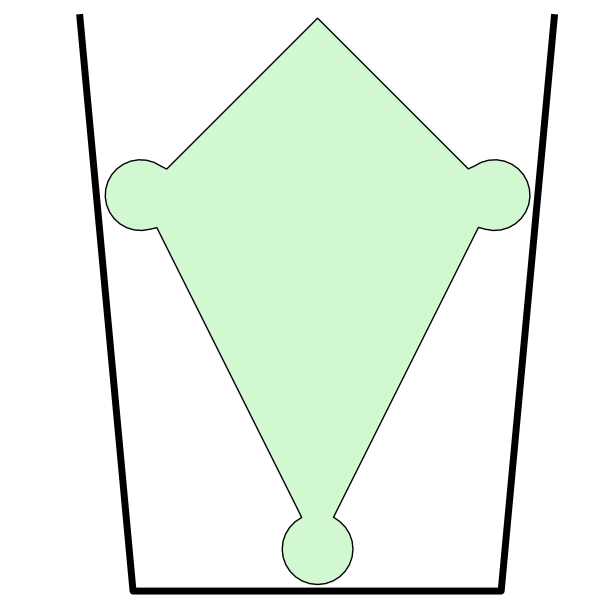
\includegraphics[width=1.5in]{figures/three_contact.png}
% \end{center}
% \caption{Peg making three contacts with the hole joint. If no error exists, these three contacts is sufficient to provide stability. }
% \label{fig:three_contact}
% \end{figure}


% When all errors are excluded, three contacts are sufficient to provide the peg stability inside the hole joint, as shown in Figure~\ref{fig:three_contact}. As no error exist, the peg cannot translate horizontally inside the hole, but only vertically up to exist the hole. Rotation of the peg, however, is not impossible geometrically. If we consider an outward pointing normal at each contact point between the peg and the hole, then a possible rotation of the peg would be that all contact points {\em slides} to the left of the original normal. 

% To prevent such a rotation, we need to make sure that if any two contact slides along the surface of the hole joint, the third contact would create a {\em pinch} situation. Because the bottom contact cannot get into a pinch situation, we will need to make sure the side contacts would create a pinch situation when sliding. Since the peg is symmetric, we can only consider one contact. Let us consider the previously mentioned sliding direction, all towards the left of the original contact normal. 

% Let the radius of the bump be $r$, the distance between the two centers of the side bumps be $2d$, and the midpoint  of the line connecting two side bump centers have distance $h$ to the center of the bottom bump center, and let that midpoint be the origin $(0, 0)$. Also, let the side of the hole slant at an angle of $\alpha$. Let us denote the rotation angle of the peg by $\beta$, the orientation difference between the center axis of the peg before and after rotation. 

% If the sliding is possible and the peg rotates an angle $\beta$, let the new coordinate of the previous origin be $(x, y)$, we will have, 

% \begin{eqnarray}
% |y| = h(1 - \cos\beta)\\
% \tan\alpha = \frac{d}{h}
% \end{eqnarray}
% which indicates that as long as $\alpha < \arctan(\frac{d}{h})$, the pinch will happen, so the rotation of the peg is not possible inside the hole. 

% However, if there exist an external force that have a projection that is along the axis of the peg pointing outwards of the hole joint, it is still possible to move the peg inside the hole. The contacts may depart from the surface, making the peg only contacting the hole at one point or even not contacting at all. We will not consider such situations since the peg-and-hole joint can never prevent such situations as there is no balancing force along the extraction direction. 

% Another important design measure of the peg joint is the length of the peg versus the width of the peg. Based on the previous analysis, even though as long as the slant of the hole satisfy the condition, the pinch can prevent peg of any rotation, this ratio can potentially affect how robust of those contacts against external forces. By robust, we mean the size of the wrench cone that can change the contacts to get into the pinch condition. If the peg and the hole are both perfectly rigid, the pinch should be able to prevent all potential forces, but in reality nothing is perfectly rigid. Therefore, the less we rely on the pinch to prevent rotation, the more stable the peg will be inside the hole. 

% Using the method introduced in~\cite{} to analyze the size of the wrench cone that can change contact modes, we can analyze the robustness of those contacts. Given the three contacts at the defined locations, the analysis show that when there is no error, the shorter the peg is, the more robust the contact will be, i.e. the smaller the wrench cone is that can move the peg contact points. 

% The result is not hard to interpret. The shorter the peg is, when a force try to rotate it, the less the side contact location will rotate, thus the more overlap it has with the original contact point, i.e. the original contact location serves as the pinch contacts. As the peg becomes longer, a small rotation of the peg will move the original contact location by a large amount, thus the original contact is no longer part of the pinch configuration. Therefore, the shorter the peg is, under perfect condition, the more robust the contacts are to external forces. 

% A shorter peg also means that the slant of the hole can be larger without giving up the pinch condition. The more gentle the slant is, the easier it is for insertion, which we will discuss in the next section. 



% \subsection{Ideal joint for insertion}

% Inserting a peg in a hole is not easy when implemented by a robot. A slight change of the orientation of the insertion can get the peg stuck along the edge of the hole, and keep applying forces along the tip of the peg will not be able to {\em unstuck} the peg. This is especially challenging when the contacts designed between the peg and hole are surface contacts. Therefore, sharp corners of the peg will easily get into a pinch situation with the edge of the hole. A slight offset perpendicular to the depth of the hole can also introduce problems, and surface contacts in this situation is again not beneficial. 

% To overcome the pinch situation to allow the tip of the peg into the hole, the edge of the hole should be vertical or even be tilted so that the bottom of the hole is wider. On the other hand, to overcome the issue with the offset perpendicular to the depth of the hole, the edge of the hole should be tilted so that the entrance should be wider. Obviously, these two conditions are contradictory, so what should be the ideal design of the hole to allow this easy insertion? 


% Many of the above issues are caused by the surface-surface contacts and sharp corners. Since we have decided to adapt point contacts rather than surface contacts, the analysis becomes simpler. A slanted edge of the hole can address most of the issues. The key would be how much slant can there be. 

% Geometrical stability dedicates that the slant cannot be more than $\arctan{\frac{d}{h}}$. To avoid insertion pinch, the slant should be smaller, while to avoid the translational offset, the slant should be larger. Question is, given the slant angle no larger than $\arctan{\frac{d}{h}}$, and the point contact design shown above, can the insertion pinch still happen? Let us assume that the insertion angle cannot be larger than $\theta$, and the translational offset cannot be larger than $\Delta$. In addition, let the friction coefficient between the peg and the hole be $\mu$. 

% To analyze the potential pinching situations, the translational offset can be dropped, as long as the slant of the side of the hole joint is consistent, which we will assume to be the case here. Based on the shape of the peg designed above, in order for a pinch-like condition to happen, the circular bump at the tip of the peg will need to be contacting the side of the hole while the other side of the hole will contact one of its side bump-contacts, as shown in Figure~\ref{fig:tilt}. 

% \begin{figure}
% \begin{center}
% 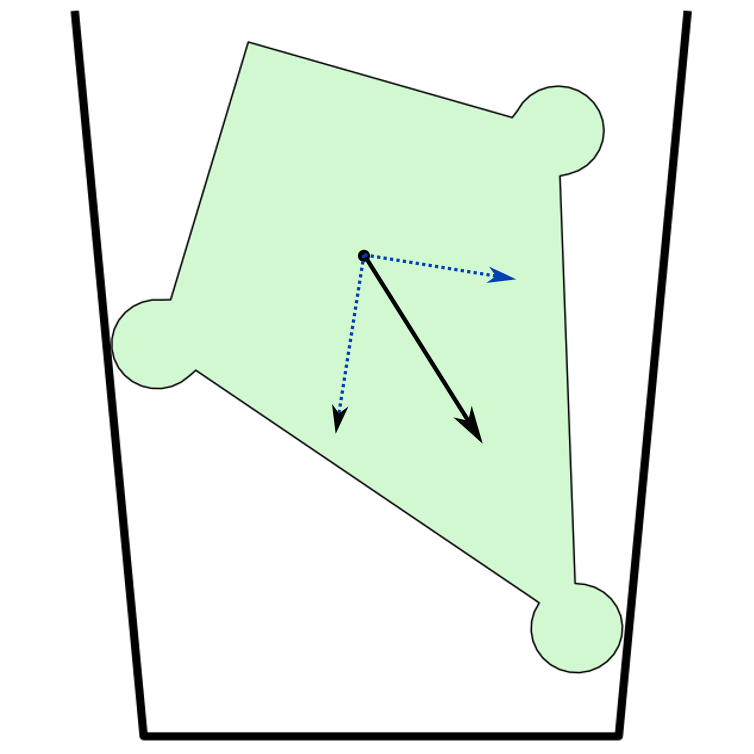
\includegraphics[width=1.5in]{figures/tilt.png}
% \end{center}
% \caption{Peg inserting into the hole with a small rotation angle of $\theta$. The tip of the peg contacts the side of the hole. }
% \label{fig:tilt}
% \end{figure}

% So, in order for the peg to be able to continue moving towards the bottom of the hole joint, we will need to have $F\cos{\frac{\pi}{2}-\theta-\alpha}\cdot\mu \leq F\sin{\frac{\pi}{2}-\theta-\alpha}$, which lead to $\theta+\alpha\leq \arctan{\frac{1}{\mu}}$. Therefore, as long as the total tilting angle is not too large, the peg should be able to continue the insertion. 

% In the illustrated insertion situation, when the condition of the total tilting angle is bounded as shown above, even when the hole becomes narrower so that the peg can no longer move deeper into the hole without rotation, because the force projection along the depth of the hole is larger than the friction between the peg and the hole, the force is sufficient to push the peg to rotate, reaching the bottom of the hole. 

% \begin{figure}
% \begin{center}
% 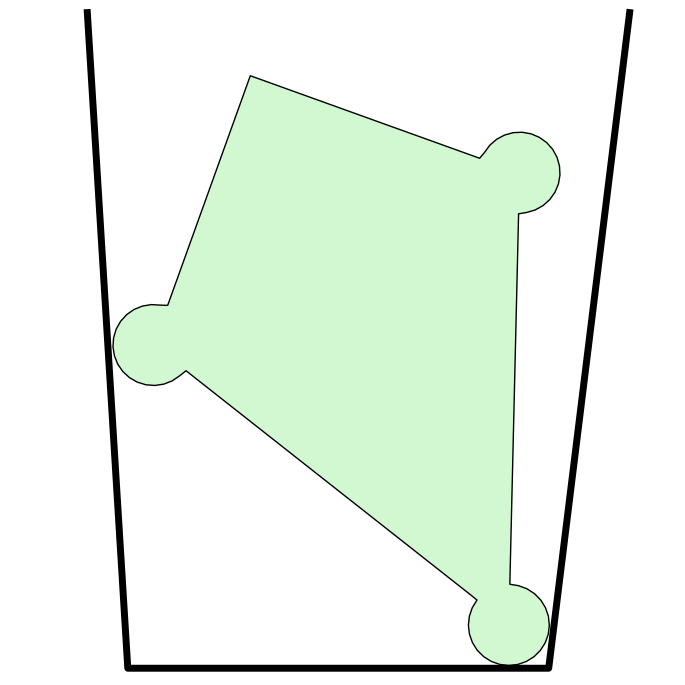
\includegraphics[width=1.5in]{figures/contact_bottom.png}
% \end{center}
% \caption{Peg inserting into the hole with a small rotation angle. The tip of the peg contacts both the bottom and side of the hole. }
% \label{fig:contact_bottom}
% \end{figure}

% Another problem rises though, based on the design shown above. When the tip of the peg keep sliding towards the bottom of the hole, once it contacts the bottom of the hole joint, as well as the right side of the hole joint (Figure~\ref{fig:contact_bottom}), the force pushing the peg may not be able to adjust the peg into the desired configuration as shown in Figure~\ref{fig:three_contact}. Such situation cannot be resolved unless an adjustment of insertion force is made, mainly, the direction of the force. This would also suggest that if there do exist a small error in the insertion angle, based on the three contact design, the  peg cannot reach the desired goal configuration, which suggests that our design needs to be modified. 

% \begin{figure}
% \begin{center}
% 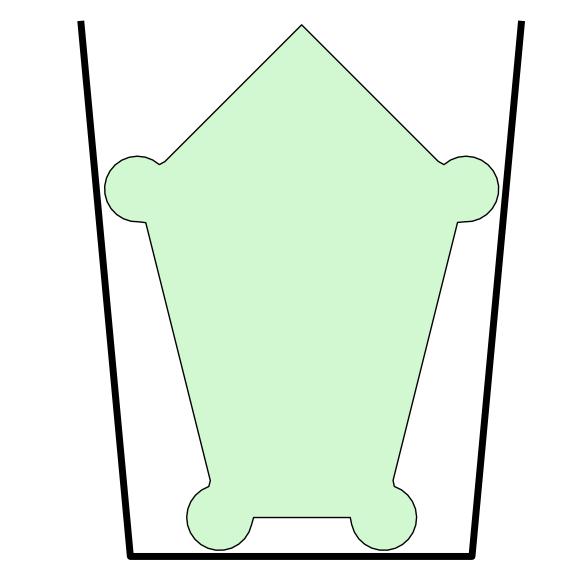
\includegraphics[width=1.5in]{figures/four_contact.png}
% \end{center}
% \caption{A redesigned peg, with four contacts in total. Two contacts at the sides of the peg, and two at the tip of the peg. }
% \label{fig:four_contact}
% \end{figure}

% The key is to avoid the situation where a single desired contact point, which has to be modeled as a circular bump on the peg, can contact two sides of the hole at the same time. Therefore, a single bump at the tip of the peg cannot be used, but a set of two contacts at the tip of the peg can successfully avoid the situation stated above, as shown in Figure~\ref{fig:four_contact}. Based on the width of the the two contacts at the tip of the peg relative to the width of the hole, the force pushing the peg into the hole can make the transition between the contact of the tip with the side of the hole, to the contact between the upper-right contact with the side of the hole. 

% Let the distance between the two tip contacts be $2w$, and recall that the depth of the peg is denoted as $H$, then the angle constraint becomes $\theta+\alpha+\arctan{\frac{w}{h}} \leq \arctan{\frac{1}{\mu}}$. The larger the distance between the two contacts on the tip, the smaller the total tilt angle can be, so we may not wish to have the distance between the two tip contacts be too large. 

% On the other hand, the smaller the distance between the two tip contacts, the harder it is to transition from the tip contacts to side contacts with the hole, as the limit of that is the single contact at the tip, which can contact both the bottom and the side of the hole and can never transition to the side contacts on the peg. 

% Because of the two contact near the tip, the goal is to never let the designed bump to make contact with two edges at once, i.e. maintaining the point contact design. But since the bump have a non-zero radius, it is always physically possible to have a small but none-zero tilt of the peg, and both contacts near the tip contacts the bottom of the hole, while one of the bump still makes contact with the side of the hole. Therefore, we need to have the bumps to have very small radius as a first constraint. Second, at the time or before the above stated situation happens, we would like to have the contacts shifted from the tip contacts to the side contacts. This leads to a relative small distance between the tip contacts, where as the tilt of the peg reduces due to the pushing of the peg into the hole, the peg can make both contacts at the side of the hole, and further push of the peg into the hole will separate the tip contact with the side wall of the hole, as shown in Figure~\ref{fig:four_contact_tilt}. 

% \begin{figure}
% \begin{center}
% 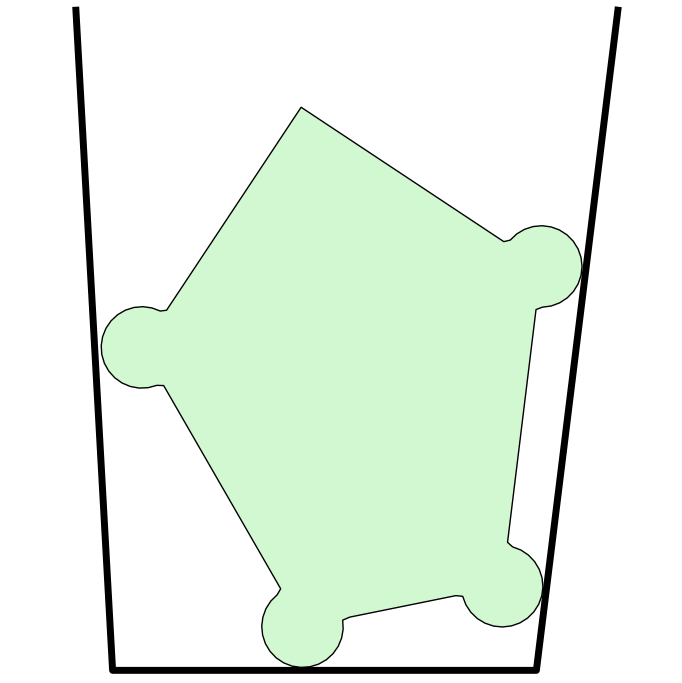
\includegraphics[width=1.5in]{figures/four_contact_tilt.png}
% \end{center}
% \caption{A tilt of the peg makes four contacts with the hole, but not yet at the desired locations. But on the side of the wall, the peg makes two contacts with the side of the hole, and further push of the peg will separate the contact between the bottom-right tip of the peg with the side of the hole. }
% \label{fig:four_contact_tilt}
% \end{figure}

% Now, putting the above analysis together. When there are no manufacturing errors, to allow successful insertions as well as stability after insertion, we should have four contacts designed with the peg, two near the tip, two on the side. 


\section{Joint design process}
\label{sec:design}


In this section, we present the details of the design process. The analysis and the design process is derived under the assumption of the existence of manufacturing error. For simplicity of analysis, the error is assumed to be uniform, and was only attached to the socket while the peg is {\em perfect}. Though the analysis of the peg and the socket are both considered in isolation, both the peg and the socket are part of a block, which is of limited size. Therefore, the size of the peg and the socket are limited with respect to the block. 

The design process for insertion and the stability after insertion are analyzed separately. In the insertion process, the main goal is for the peg to be fully inserted into the socket, regardless of the initial configuration or the intermediate stages the insertion has to go through. The initial insertion configuration of the peg is assumed to be within a bounded error of the perfect insertion location and orientation, simulating the sensing error and grasping error during assembly. The success of transition between different stages is the key to reaching the final inserted configuration, which we refer as a {\em sink}. The analysis of the insertion stage focus on ensuring the success of these transitions. 

After the insertion, the peg may move within the socket under external disturbance, if the manufacturing error exists. As the relative translation of the peg within the socket is unavoidable, the main goal for the peg stability is to achieve the minimum possible rotation within the socket. A design change that reduces such rotation is considered an improvement, and finding such changes is the goal for the stability analysis. 

As the design of the joint consists of two parts, the peg and the socket, we will consider the change of one component of the joint only for each process. In the insertion stage, we will treat the peg as a fixed design, and study how the socket can be changed to maintain the success of insertion transitions and possibly improve the ease of transition. In the stability analysis after the insertion, we will treat the socket as a fixed design, and change the peg shape, i.e. the contact locations between the peg and socket to improve the stability. Then, through the iterations of the insertion and stability analysis, we can find the {\em best} design that is beneficial to insertion and stability. 

% uniform error



% The problems rises when manufacturing error starts to be introduced. A few assumptions needs to be made before we go any further. First, let the peg and the hole both be attached to a wide block, so that when peg is fully inserted inside the hole, the edges will make contact. Second, let the error only occurs on the peg and let the hole be unchanged. Third, let the errors be uniform everywhere on the peg and the error reduces the size of the peg. 

% The first assumption is placed to simulate real assembly scenarios. The second assumption allow us to analyze the change of contacts and how the peg can be moved inside the hole relatively. The third assumption is reasonable because usually the blocks can be made with molds, and exceeding the allowed size is impossible. 

% With the given assumptions, we will show how to place the contacts to best reduce uncertainties and remain stable, both during insertion stage and after insertion. 

\subsection{Mode of contacts and transitions}

% The insertion process of the peg into the socket may involve the points on the peg contacting different edges of the socket at different {\em stages} of the insertion, The goal for the insertion is clear: the peg must be fully inserted into the the socket so that if there is no error in the manufacturing, each point on the peg should contact the designed edge on the socket, even when the initial insertion angle and placement may contain bounded error. 


% However, as each contact between a point on the peg and an edge on the socket introduces an additional constraint, the straight optimization of the socket and peg design may involve different set of constraints at different stage of the insertion. The result of the optimization under any given set of constraints may not extend to other stages. We need to find how the effect of the design changes may affect across different stages of the insertion. 


During the insertion, the peg may contact the socket along different edges at different locations. Maintaining the contacts at different edges requires different set of constraints. Therefore, to ensure the success of insertion, there are different sets of constraints one needs to maintain, depending on the {\em stage} of insertion. This makes the straight optimization of joint design difficult to model. 

On the other hand, the different sets of constraints can be considered separately, if we discretize the insertion process. We define {\em Mode of Contacts} as a collection of point-edge pairs that are in contact, and to each point-edge pair that is in contact as a {\em Contact Pair}, denoted as $CP(i, j) = \{p_i, e_j\}$. We use $p_i$ to denote the $i$th point on the peg following a counter-clockwise order, and $e_j$ to denote the $j$th edge on the socket in the counter-clockwise order. We also denote the Mode of Contact as $MoC(k) = \{CP(a, b), CP(c, d), \ldots\}$. Then, the entire insertion process can be described as a directed graph when the insertion is guided by a known force. 

In this paper, we only consider the Contact-Pair as the pair containing a point on a peg and an edge on the socket. For simplicity, the points on the peg can be joined by different designs (curves) to avoid any contact between the socket edges other than the bounded number of designed contact points. In addition, a point on the peg contacting two adjacent edges on the socket, i.e., a point-point contact, can be viewed as two contact pairs. Therefore, the Contact-Pair defined above is the fundamental unit for analyzing the Mode of Contact in the peg-socket relation. 

We will first find the set of all valid Mode of Contacts (MoCs). In order for a Mode of Contact to be valid, all the containing Contact Pairs need to be valid for the given peg and socket, and a valid configuration must exist to allow the set of Contact Pairs to co-exist. We adapted a bottom up approach to find the valid MoCs: identifying all valid Contact Pairs (CPs), and find all combinations of CPs to form potential valid MoCs; for each of the candidate valid MoC, we test if there exist a valid configuration allowing the set of CPs co-exist. 

% Then, for all the valid Contact Pairs, we can find all possible combinations of the Contact Pairs and test the validity of each combination, and the resulting valid combinations are the valid Mode of Contacts between the given peg and socket geometry. The valid Mode of Contacts can also be found by translating and rotating the peg within the socket, but as the rotations and translations is a continuous process, the approach may be slow and inaccurate though easy to implement. 

The MoCs along cannot fully describe the insertion process, as the insertion process also involves the transition between different modes. To find out whether a transition between two Mode of Contact under a given force is possible, we can find the acceleration direction under the insertion force, and the location of the different CPs between the two modes. If the acceleration / moving direction can lead to the contact or the removal of the corresponding point-edge pairs, then the transition is valid, otherwise not. 

% For example, Figure~\ref{fig:cm_increase} shows an example of a possible transition between two MoCs, from $MoC(20)$ to $MoC(41)$, for the given five-edge five-contact joint design. Insertion force ($F$) generates different reaction forces for different CPs, which are denoted as $F_{CP(i, j)}$. 

% $F_t$ is the joint force on The point of the different Contact Pair $CP(5, 5)$, e.g. joint force on $p_5$. Along the force $F_t$, $p_5$ in $MoC(20)$ would move to $e_5$, so the transition of $MoC(20)$ to $MoC(41)$ is valid.

% \begin{figure}[h]
% \begin{center}
% 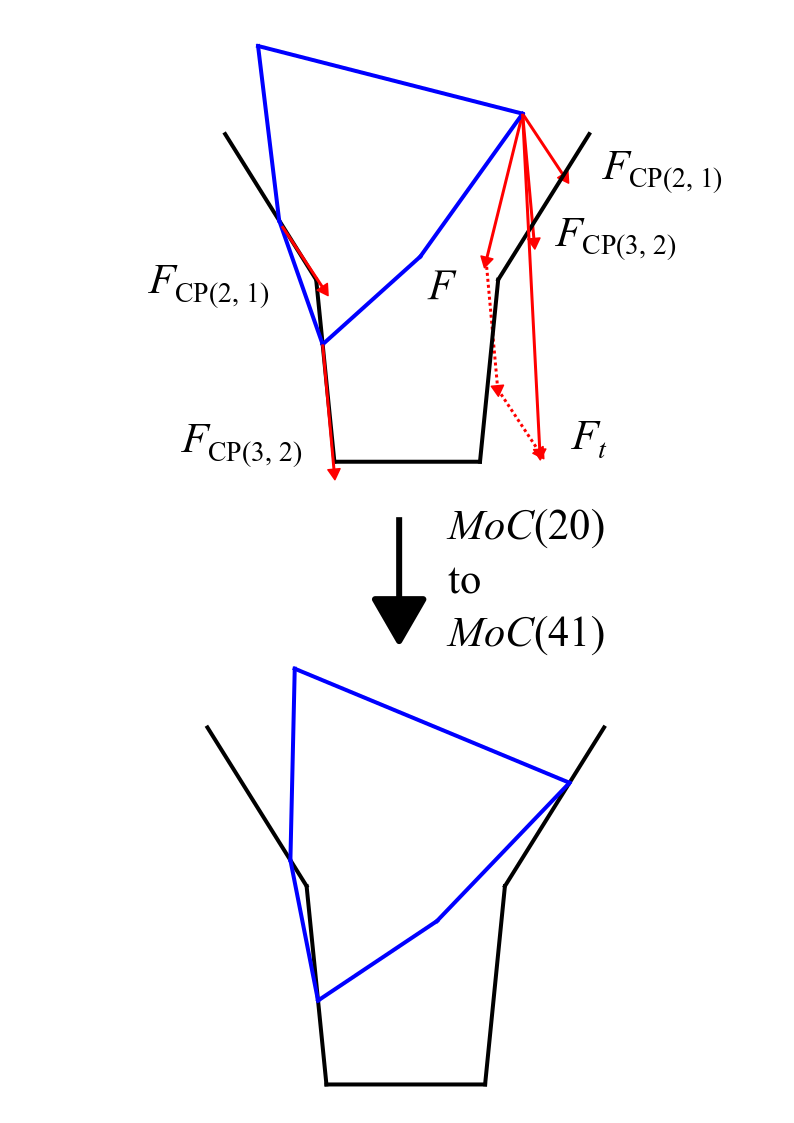
\includegraphics[width=2.5in]{figures/cm_increase.png}
% \end{center}
% \caption{Force diagram for $MoC(20)$ transfering to $MoC(41)$. }
% \label{fig:cm_increase}
% \end{figure}

% Therefore, in this paper we only consider the transition between {\em neighbors}.

There is a huge number of possible transitions among all valid MoCs. For simplicity, we can view a potential transition between arbitrary two modes as a sequence of transitions between two {\em adjacent modes}. Given $MoC(i)$ and $MoC(j)$, if the difference between the two MoCs is $d$ Contact Pairs $CP_k(a, b), 1\leq k\leq d$, then we refer these two MoCs as {\em $d$-neighbors}. We can show that arbitrary {\em valid} transition between two MoCs during insertion can be decomposed to either a sequence of transitions between $1$-neighbor MoCs, or a special transition between $k$-neighbors where $k$ can be uniquely computed for given peg and socket, and there can only exist a bounded number of special transitions. In addition, add a special MoC with no contact pairs. 

We therefore can define a directed graph $G = (V, E)$, where $V$ is the set of valid MoCs, and $E$ are the valid transitions between neighbor modes or among special modes. We refer this graph as the Contact Mode Transition (CMT) graph. Then, for each vertex on the graph, the set of constraints describing the relation between peg and socket is of fixed number. 

% Given $MoC(n)$ and $MoC(m)$, if the Contact Point $p$ is unique for all Contact Pairs in the difference set between $MoC(n)$ and $MoC(m)$, we define $MoC(n)$ and $MoC(m)$ are neighbors. It means there is only one point contact or remove between neighbors, though it may increase or decrease one or more Contact Pairs (point-point case).

% Set $MoCs$ as nodes (To complete the graph, we also define non-contact mode as a special node) and the transition as directed edge. We can find a CMT graph, and the insertion process is discretized into different Modes. Each mode consists of a fixed set of point-edge constraints, so that the analysis becomes simpler, as well as optimization. 

% \subsection{Constraints for the peg successfully inserted into the socket}

% \subsection{Capturing the peg}

To simulate the sensing error during automated assembly, we introduce a $\Delta x$ and a $\Delta\phi$ during insertion process. The two values denote the maximal offset along $x$ axis and the maximal rotation allowed at the beginning of the insertion, which is bounded by the precision of the sensing technology. Under such initial error, we would like the designed peg to still be able to be inserted into the socket. One of the necessary condition for the success of insertion is the peg not contacting any edge outside the socket, which we refer to as the {\em capture} of the peg. In the remaining section of paper, for simplicity, we connected contact points on the peg with straight edges, but the actual design may require these connection to be curved to avoid undesigned contacts. 

% In the insertion process, there is an important step called {\em capture}, which is the prerequisite for CMT graph. Only the peg is captured by the socket, the peg can be inserted correctly. Therefore, designed peg-socket joint should keep peg captured by the socket under the rotation angle $d\theta$ and transition error $dx$ for the manipulator. 

% If there is no point of the peg contact outside the socket during insertion, we define the peg is captured. In the definition, we do not take edges into consideration, since edges of the peg can be curve. 

Figure~\ref{fig:not_capture} shows an example of the peg not captured by the socket. In the given example, $p_1$ contacts the outside the socket during insertion, which can prevent further insertion. However, by rotating the top-left edge of the socket, the peg can be captured in Figure~\ref{fig:captured} with same $\Delta x$ and $\Delta\phi$. After the peg is captured by the socket, we can derive its CMT graph. 
% Since the opening angle of the socket is large enough, $p_1$ of the peg would never contact outside the socket during insertion.

\begin{comment}
Given manipulator rotation angle and transition error $d\theta$ and $dx$. Let ${2\theta}_{up}$ be the angle between two upper edges of peg, and ${2l}$ be the top edge length of peg. Denote socket opening angle and opening distance as $2{\theta}_{op}$ and $2{L}$, respectively. 

As shown in Figure~\ref{fig:capture}, socket can not capture the peg if
\begin{eqnarray}
l\cos{d\theta} + dx > L\\
\theta_{up} + {d\theta} > \theta_{op}
\end{eqnarray}
here, ${l}={L}\times{t}_{up}-\epsilon$. Keeping ${L}$ unchanged, we have 
\begin{eqnarray}
{t}_{up}>\frac{L-dx+\epsilon\cos{d\theta}}{L\cos{d\theta}}\\
\theta_{op}<\theta_{up} + {d\theta}
\end{eqnarray}
which indicate that, to make peg captured under the maximum error, we should make 
${t}_{up}\le\frac{L-x_m+\epsilon\cos\theta_m}{L\cos{\theta}_m}$ or $\theta_{op}\ge\theta_{up} + {\theta_m}$. 
\end{comment}

\begin{figure}[t]
\begin{center}
\begin{subfigure}[t]{0.24\textwidth}
\begin{center}
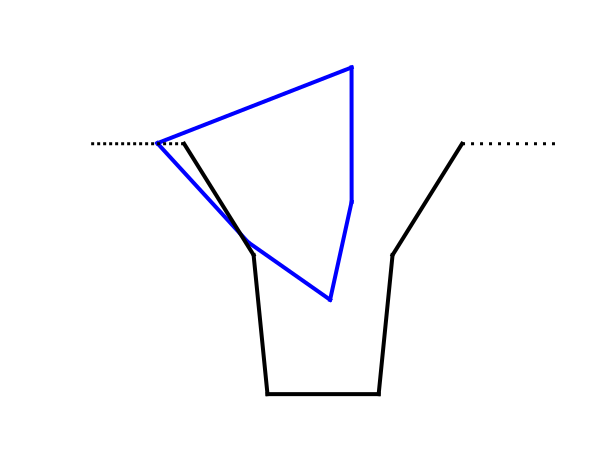
\includegraphics[height=1.3in]{figures/not_capture.png}
\end{center}
\caption{The peg is not captured by the socket. }
\label{fig:not_capture}
\end{subfigure}
\begin{subfigure}[t]{0.24\textwidth}
\begin{center}
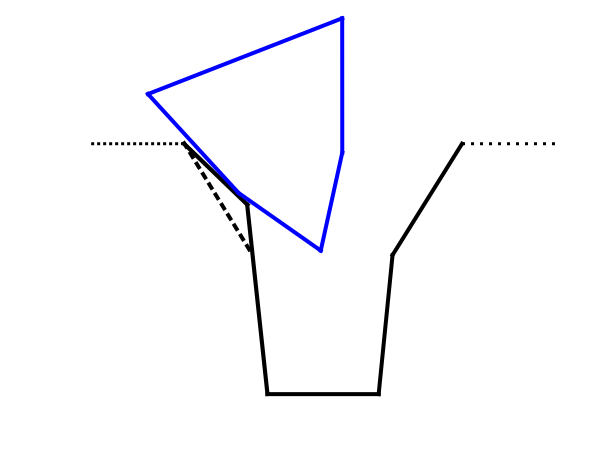
\includegraphics[height=1.3in]{figures/captured.png}
\end{center}
\caption{The peg is captured by the socket.}
\label{fig:captured}
\end{subfigure}
\caption{An example of peg not captured by the socket, and how the socket can be changed to guarantee the capture. }
\label{fig:capture}
\end{center}
\end{figure}

% In this way, for a given peg-socket joint, if we have the bound of rotation angle $\theta_m$ and the transition error $x_m$ for the manipulator, we could find the {\em Limit Opening Angle} (LOA) of the socket to keep the peg always captured. 

Define a {\em sink} on the CMT graph as a vertex that either has only in coming edges, or has outgoing edges and incoming  edges with another {\em sink}. A insertion process can be considered successful only if the CMT graph has sinks, but the inverse statement is not true, as some sinks are not desired. For example, a CMT graph for a five-edge socket and a five-point peg is shown in Figure~\ref{fig:insertion_graph}, four sinks are identified, and are shown in Figure~\ref{fig:5_5_sink}. The sinks shown in Figure~\ref{fig:5_5_sink2} and~\ref{fig:5_5_sink3} are not desired, as the peg is not fully inserted and by definition the peg cannot get out of the MoC under the insertion force. 
% Weifu Question: how to identify the desired sinks or undesired sinks automatically? 
% discussion; 

% If there exist {\em sinks} in the CMT graph, which means the peg can get a stable state eventually under the configuration force, that is, successful insertion. To keep the insertion successful in the iterative optimization, the peg-socket design should not break the sink in each iterate, which introduces another constraint besides capture for insertion. 

% Figure~\ref{fig:insertion_graph} is an insertion CMT graph for a five-point peg and five-edge socket joint. In which, there are 46 nodes including 45 contact state ($MoC(1)- MoC(45)$) and 1 non-contact state ($MoC(46)$). From the graph, we can find four sinks, e.g., $MoC(36)$, $MoC(37)$, $MoC(41)$, and $MoC(42)$, which are shown in Figure~\ref{fig:5_5_sink}.  
\begin{figure}
\begin{center}
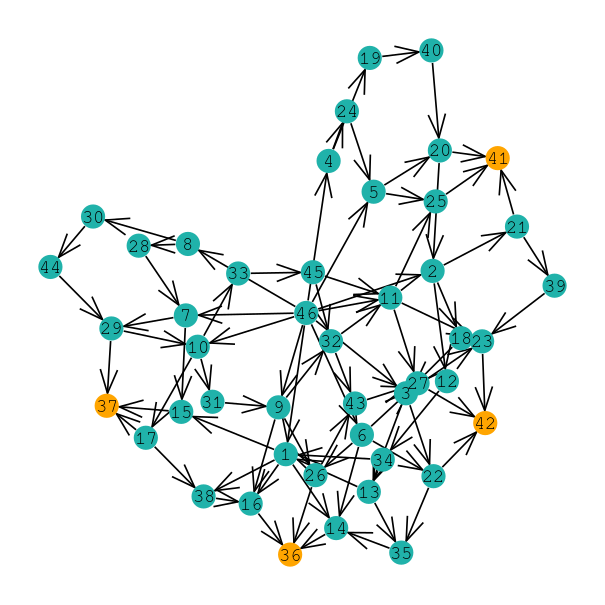
\includegraphics[width=3in]{figures/insertion_graph.png}
\end{center}
\caption{The insertion graph of a five-point and five-edge peg-socket joint. }
\label{fig:insertion_graph}
\end{figure}

% It's reasonable to have four different sinks, since the rotation angle $d\theta$ and the transition error $dx$ are both uncertain. Though both $d\theta$ and $dx$ have a bound, the change of $d\theta$ and $dx$ within the bound would lead to different initial configurations of the peg. Therefore the peg would transfer to different stable states. Here, sink 1 and sink 4 are desired sinks , while sink 2 and sink 3 are sinks we want to avoid.

\begin{figure*}
\begin{center}
\begin{subfigure}[t]{0.24\textwidth}
\begin{center}
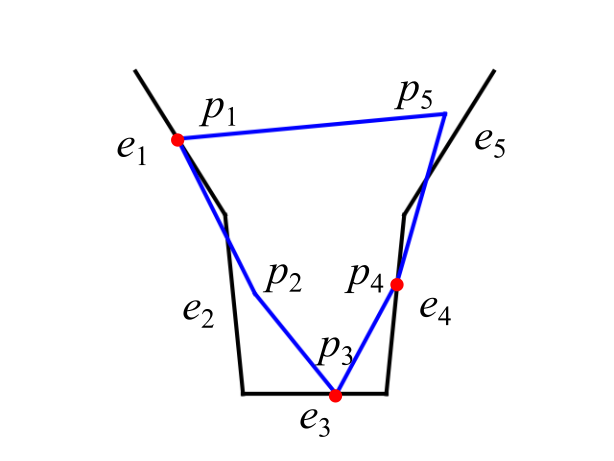
\includegraphics[height=1.3in]{figures/5_5_sink1.png}
\end{center}
\caption{Sink 1. $MoC(36)$ with $CP(1, 1)$, $CP(3, 3)$ and $CP(4, 4)$.}
\label{fig:5_5_sink1}
\end{subfigure}
\begin{subfigure}[t]{0.24\textwidth}
\begin{center}
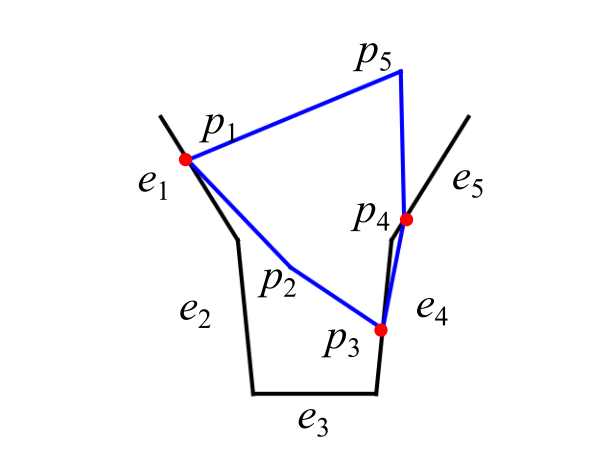
\includegraphics[height=1.3in]{figures/5_5_sink2.png}
\end{center}
\caption{Sink 2. $MoC(36)$ with $CP(1, 1)$, $CP(3, 4)$ and $CP(4, 5)$. }
\label{fig:5_5_sink2}
\end{subfigure}
\begin{subfigure}[t]{0.24\textwidth}
\begin{center}
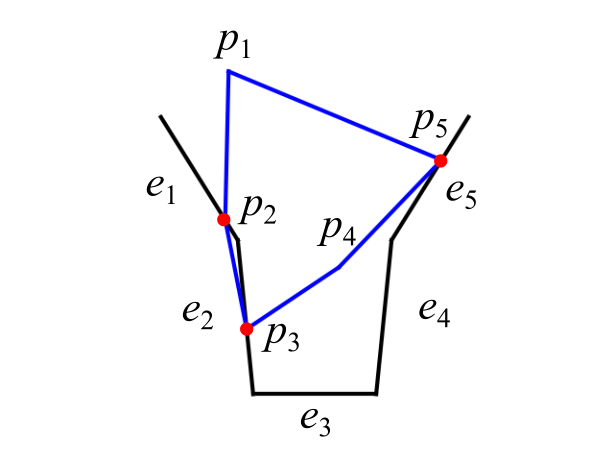
\includegraphics[height=1.3in]{figures/5_5_sink3.png}
\end{center}
\caption{Sink 3. $MoC(41)$ with $CP(2, 1)$, $CP(3, 2)$ and $CP(5, 5)$. }
\label{fig:5_5_sink3}
\end{subfigure}
\begin{subfigure}[t]{0.24\textwidth}
\begin{center}
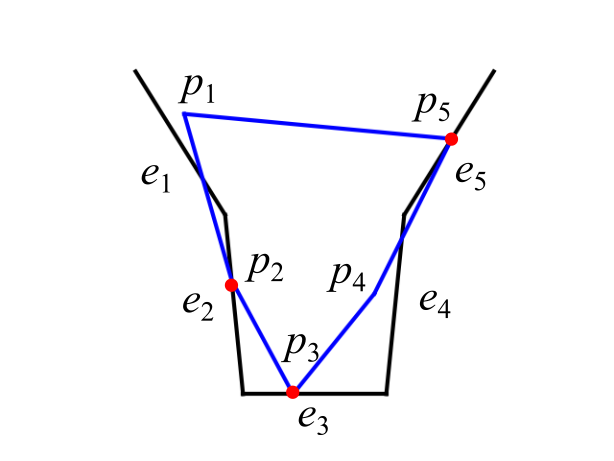
\includegraphics[height=1.3in]{figures/5_5_sink4.png}
\end{center}
\caption{Sink 4. $MoC(42)$ with $CP(2, 2)$, $CP(3, 3)$ and $CP(5, 5)$.  }
\label{fig:5_5_sink4}
\end{subfigure}
\end{center}
\caption{Sinks of an insertion CMT graph for joint with five-point peg and five-edge socket. }
\label{fig:5_5_sink}
\end{figure*}


% comment Weifu: Redraw this figure with labeled edges and contact points on the peg, you can edit the figure with inkscape. This edit is needed as you referred contact pairs with indexes of edges and points. 

% For each sink, we keep the $MoC$ and the corresponding configuration force unchanged but rotate the contact edge of each contact pairs in the $MoC$. If the force between the contact pair become zero under the edge rotation angle and the configuration force, it means the rotation would break transition to the sink; the rotation angle is the {\em Limit Edge Rotation Angle} (LERA) for the corresponding edge. 

% From the analysis above, we have LERA and LOA as two constraints for insertion. The former is affected by the configuration force of the sink and the coefficient of friction $\mu$, while the later is affected by $\theta_m$, $x_m$ and the peg design.


% HERE, weifu
% The edge of the socket can be rotated to affect the insertion process, and possibly change the CMT graph.
% mvoe this to later, where the design process is presented as a procedure. 




% \subsection{Optimizing the stability for the peg and socket}
\subsection{Stability after insertion}

Another important criteria for a good peg-socket design is how stable the peg will be in the socket after insertion, under external disturbances and subject to manufacturing error. Under the assumption of an uniform error, the translation of the peg inside the socket after insertion is unavoidable regardless of the design, but the possible rotations can be reduced by changing the designs. 

Intuitively, given the same amount of error $\epsilon$ between the peg and the socket, the longer the peg is, the less rotation is possible after insertion. However, as the peg and the socket are both part of a block, which has bounded size, we have to assume the maximum depth of the socket is bounded. The question then becomes, how will the different designs of peg and socket reduce possible rotations after insertion? 

% Besides insertion, another import evaluation for the designed joint is the stability, e.g., the {\em Maximum Rotation Angle} (MRA) of the peg in the socket under the uncertain force. The optimization of stability is to minimal the MRA of the peg in the socket.

% However, straight optimization is also unsuitable for computing MRA due to the change of constraints with peg "rocking" in the socket. Geometry rotation method does not work well either, since it needs to loop over a large number of fulcrums for rotation. Therefore, in this section, we also discretize the "rocking" process as MoCs. By comparing the MRA of each MoC, we can fund the MRA of the peg in the socket. 

% Different from insertion, to keep peg in socket, we add a top edge closing the socket. In reality, the peg should be attached on block base, which is equivalent to the top edge. This edge would add an additional constraint to optimization, therefore getting different MoCs. Some MoCs would become invalid such as sink 2 in Figure~\ref{fig:5_5_sink2} and sink 3 in Figure~\ref{fig:5_5_sink3}, since they do not satisfy the additional constraint. Besides, consider the peg in socket would rock under the force from all directions rather than the stable configuration force in insertion, the transition between any pair of neighbors should be valid. So we find a different CMT graph from insertion as shown in Figure~\ref{fig:rocking_graph}, which has no sink. Then, the state of the peg in "rocking" process is therefore discretized to MoCs in the graph, so there must exit one MoC whose MRA is the MRA of the peg in the socket.

We again discretize the possible motions of the peg in the socket after insertion based on different Mode of Contacts (MoCs). The key observation is that, there exist a partial order of all the valid MoCs, based on the possible rotations of the peg. For example, consider the two Modes of Contact shown in Figure~\ref{fig:5_5_sink1} and~\ref{fig:5_5_sink2}, the MoC shown in Figure~\ref{fig:5_5_sink2} will always have a larger rotation compared to the MoC shown in Figure~\ref{fig:5_5_sink1}. Based on this derived partial order, we therefore only need to analyze the MoCs with the highest order, i.e. the largest possible rotation. In addition, we do not want to consider the scenarios where the peg has moved away from the socket, thus we will add a {\em virtual cap} near the entrance of the socket. 

\begin{figure}[t]
\begin{center}
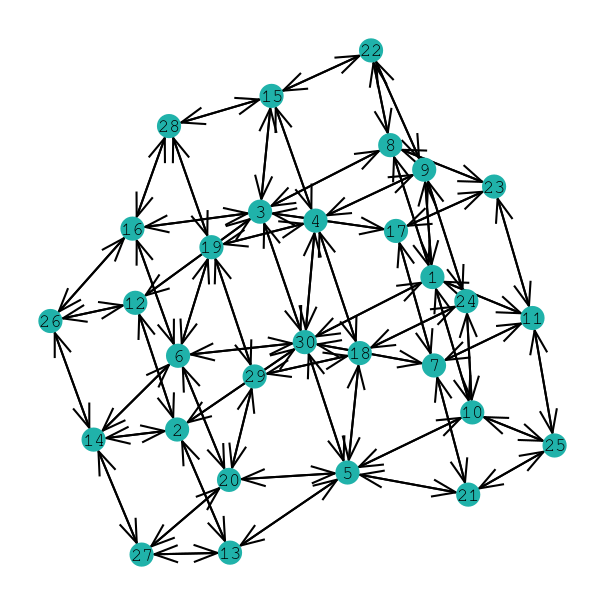
\includegraphics[width=3in]{figures/rocking_graph.png}
\end{center}
\caption{The CMT graph of the peg in socket. }
\label{fig:rocking_graph}
\end{figure}

% To simplify computing the MRA further, we introduce the partial order of MoCs. If all contact pairs of $MoC (n)$ are in $MoC (m)$, we denote $MoC (m)$ as the partial order of $MoC (n)$. Consider the rotation of the MoC would break as a new point contacting the socket, that is, a new contact pair increasing, which means the MRA of the MoC is no larger than the MRA of its partial order. Therefore, we can obtain the MRA of the peg in the socket by just comparing the MRA among partial orders.

\begin{comment}
\begin{figure}
\begin{center}
\begin{subfigure}[t]{0.24\textwidth}
\begin{center}
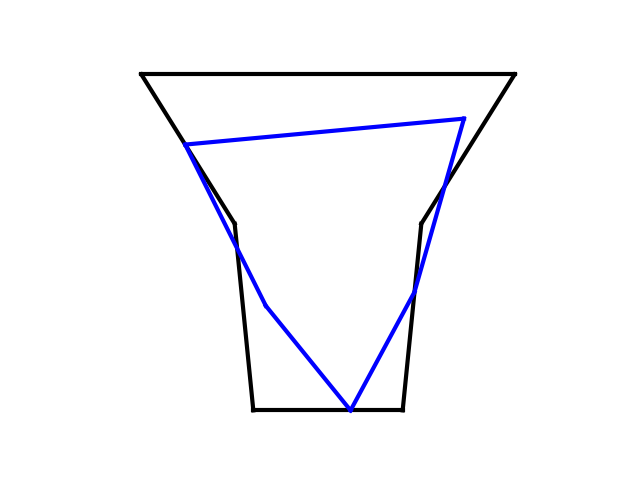
\includegraphics[height=1.3in]{figures/5_5closed_sink1.png}
\end{center}
\caption{Sink1. Contact mode with three contact pairs, e.g, $cp(1, 1)$, $cp(3, 3)$ and $cp(4, 4)$. }
\label{fig:5_5closed_sink1}
\end{subfigure}
\begin{subfigure}[t]{0.24\textwidth}
\begin{center}
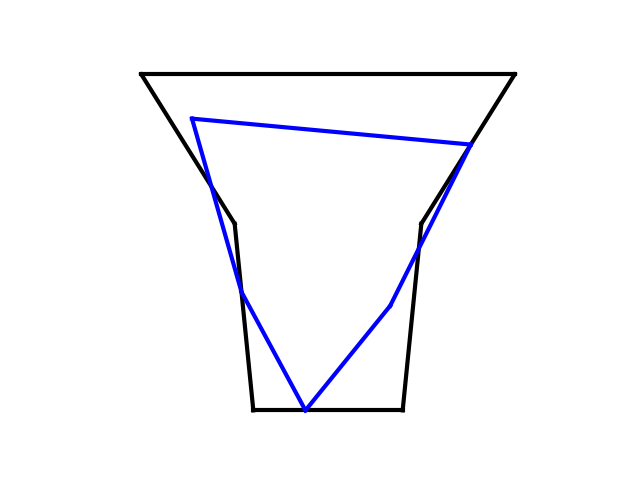
\includegraphics[height=1.3in]{figures/5_5closed_sink2.png}
\end{center}
\caption{Sink2. Contact mode with three contact pairs, e.g, $cp(2, 2)$, $cp(3, 3)$ and $cp(5, 5)$. }
\label{fig:5_5closed_sink2}
\end{subfigure}
\caption{Sinks of five points peg in closed five edges socket joint motion graph. }
\label{fig:5_5closed_sink}
\end{center}
\end{figure}
\end{comment}

% Figure~\ref{fig:5_5rotate} shows two MoCs with maximum MRA. The maximum MRA means these two MoCs are most unstable states for the peg in the socket. The reduce of the MRA of these two MoCs means the reduce of the MRA of the peg in the socket. Though the MoC with maximum MRA may change, we can find it and reduce its MRA in each iteration. In this way, the gradient of the stability of the peg in the socket is actually to reduce the MRA of the MoC with maximum MRA iteratively. 

% \begin{figure}
% \begin{center}
% \begin{subfigure}[t]{0.24\textwidth}
% \begin{center}
% 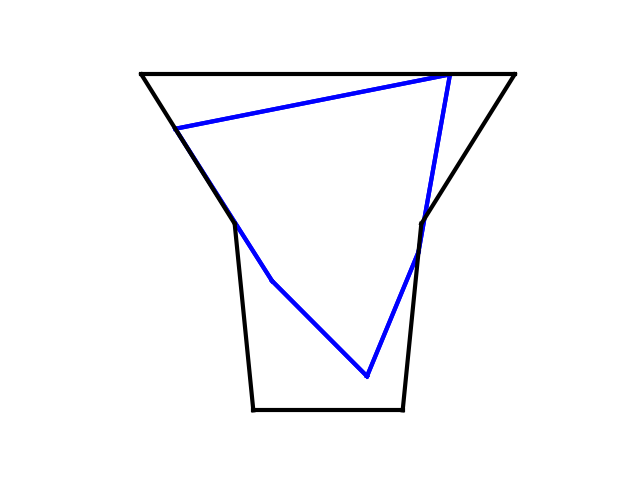
\includegraphics[height=1.3in]{figures/5_5rotate1.png}
% \end{center}
% \caption{The MRA of MoC with $CP(1, 1)$, $cp(4, 4)$ and $CP(5, 6)$.}
% \label{fig:5_5rotate1}
% \end{subfigure}
% \begin{subfigure}[t]{0.24\textwidth}
% \begin{center}
% 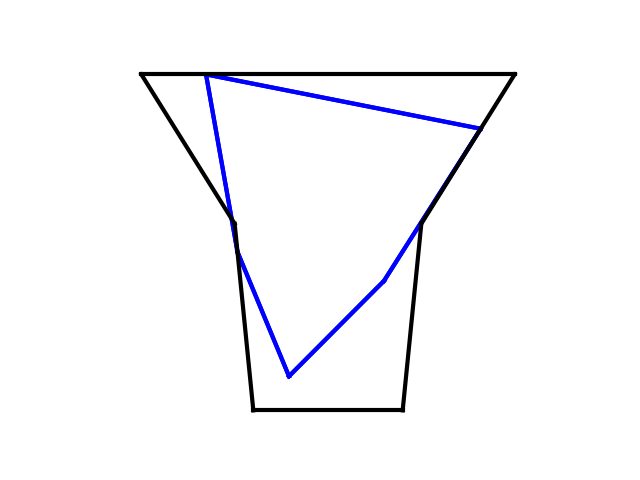
\includegraphics[height=1.3in]{figures/5_5rotate2.png}
% \end{center}
% \caption{The MRA of MoC with $CP(1, 6)$, $cp(2, 2)$ and $CP(5, 5)$.}
% \label{fig:5_5rotate2}
% \end{subfigure}
% \caption{Two most unstable MoCs. }
% \label{fig:5_5rotate}
% \end{center}
% \end{figure}

Let us define a contact point on the peg as a function of $s$, the length along a given socket edge. Then, the design of the peg becomes a collection of pairs, $(i, s)$, where $i$ denotes the designed contacting edge for the given contact point, and $s$ is the distance along the edge following the counter-clockwise direction. This definition is only valid when no error is introduced, i.e. the design for the perfect peg and socket. 

Based on the previously derived partial order, we analyze the MoCs with the highest order, and study how does the change of $s$ can affect the rotation angle of the peg inside the socket after insertion. Then, we can effectively find a direction ({\em gradient}) of contact-point (on the peg) motion that will reduce the possible rotation. Paired with the socket-edge rotation direction that can preserve (or break) the insertion transition, we can derive the following design procedure to find the {\em best} design for the joint. 

% If there is no error for the socket, the peg should be aligned into the socket without any rotation and all points of the peg should contact the edge. Moreover, there should not be any redundant point of the peg that does not contact the edge or contacts the same edge  as aligned successfully. Therefore, we can define the point of the peg by the relative location $t$ ($0 \le t \le 1$) on the edge of the socket so as to define a peg. For example, $t (i,j) = 0$ and $t(i,j) = 1$ represent the point $p_i$ is on the start point and the end point of the edge $e_j$, respectively. However, if there is an error $\epsilon$ for the socket, the point of the peg should be initialized inside the socket and definition of $t$ should be extended to the projection of the point to the edge. Generally, the initial peg is defined by the projection of point $t$ and the socket error $\epsilon$.

% Following the definition above, for a set of contact pairs, if we move the location of contact point along the contact edge, e.g., changing $t$, the design of the peg is also changed but remain the contact pairs. In this way, find the MoC with maximum MRA, then change $t$ of the contact points in the contact pairs, we can obtain the influence of $t$ to the MRA. Then, in each iterate, the peg can be optimized by changing $t$ along the direction that reduce the MRA. 

% In this way, the gradient and constraints for iterative optimization are obtained. Notice that all the analysis above are based on CMT graph. Therefore, in the optimization process, the CMT can not be broken. Consider the stability CMT graph is the subgraph for the insertion CMT graph, we choose the insertion CMT graph as a new constraint for iterative optimization. However, with the design of the peg-socket joint changed to a degree, the insertion CMT graph would also change. So for the new design, we set the new insertion CMT graph as the new constraint and do iterative optimization again.   

\subsection{Design procedure}

%  needs to be in more detail
% possibly put in an algorithm block? 

% The iterative optimization can be seen as the prediction and update for the joint design. The joint design are predicted by changing gradients and updated only as it satisfying insertion. The main steps are as follows:
% \begin{enumerate}
% \item For a given peg and socket, find the MoCs and the insertion CMT graph, if there is no MoCs or the insertion CMT graph, return the updated joint design; otherwise go to the next step.

% \item Predict the joint design by rotating socket edge. If the insertion CMT graph was broken, return to the step one; else if the peg can be captured and inserted successfully, update the joint design and go to the next step; otherwise return the updated joint design. 

% \item Find $\Delta t$ that can reduce the MRA of the peg in the socket. Let $t = t + \Delta t$, given limit $\lambda$, if $\lambda < t < 1 - \lambda$ return the updated joint design; else predict the joint design by changing the peg according to $t$. If insertion CMT graph was broken, return to step one; otherwise go to the step two.

% \end{enumerate}


Combining the analysis for the peg and the socket design, we propose the following design procedure. 

\begin{enumerate}
\vspace{-1em}
\item Input: an initial (arbitrary) design of $m$ edges (socket) and $n$ contact points (peg); friction coefficient $\mu$, and a force magnitude $|F|$; 
\vspace{-1em}
\item Find all possible CPs and MoCs for insertion, generate the CMT graph for insertion ($G_I$); 
\vspace{-1em}
\item Identify sinks, if undesired sinks exist, find edges moving directions that will remove them as sink, and change the design, until no undesired sink exist on the CMT graph; 
\vspace{-1em}
\item For each transition, identify the direction of socket edge rotation direction that will break the transition; 
\vspace{-1em}
\item Generate the CMT graph for stability $G_S$, generate the partial order for nodes; 
\vspace{-1em}
\item For each of the nodes with the highest order, find the contact-point gradient for reducing rotation;
\vspace{-1em} 
\item While $G_I$ remains the same and the rotation angle reduction $\Delta\phi$ is larger than $\delta$, the change of the edge angle or the change in $s$, iteratively move the points and rotate the edges to reduce the possible rotation after insertion; output the final design; 
\vspace{-1em}
\item If the $G_I$ is changed, compute the new insertion CMT graph $G'_I$, see if the new graph contains undesired sinks, if no, repeat the process for $G'_I$ starting from step 4; 
\vspace{-1em}
\end{enumerate}



% Given a peg-socket joint with five points and five edges, we get its optimal design as shown in Figure~\ref{fig:best_5_5_joint}. The MRA of the peg reduced with the $t(1,1), t(5,5) \to 0$ and $t(2,2), t(4,4) \to 1$. That is, the peg is more "filling" the socket, the joint is more stable.
Using the procedure described above, with $m = 5$ and $n=5$, we can find the following design show in Figure~\ref{fig:best_5_5_joint}. The blue shape is the initial input, while the red shape is the peg design output by the procedure above. In the process, we maintained an uniform error of $\epsilon$ on the socket. 


The best design for the joint overall may not share the $m$ and $n$ imagined by the user. Therefore, the procedure above should be put inside a loop that test different $m$ and $n$. However, we do not need to test $m$ and $n$ as two independent variables, as $n$ cannot be too different from $m$. If $|m-n| \geq 2$, then, there exist either two or more edges on the socket with no active contact points in the inserted configuration, or there exist two or more contact points on the peg that contacts along the same edge. The non-contact edge is redundant as they do not provide additional constraint on the rotation, and the co-linear contact points are redundant as one of the contact point will provide no constraint when rotated, leaving some contact points with no effect at all. Therefore, we only need to consider the case where $|m-n| < 2$. Also, as six contacts are sufficient to immobilize arbitrary planar object, we only need to test $m$ up to $6$, and no less than $3$. Therefore, the complete design procedure will be the above presented procedure nested inside a loop over $m$ and $n$. 


\begin{figure}[t]
\begin{center}
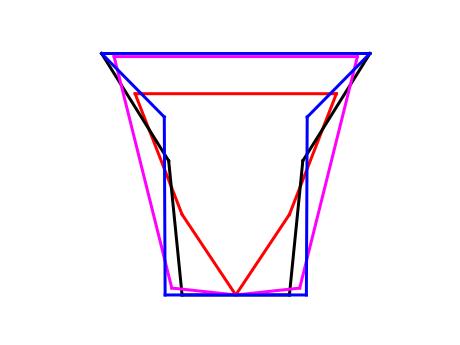
\includegraphics[width=2.3in]{figures/best_5_5_joint.png}
\end{center}
\caption{Optimized peg-socket joint design (red and brown) and given peg-socket joint (blue and black) with five peg points and five socket edge. }
\label{fig:best_5_5_joint}
\end{figure}

When the number of edges on the socket exceed four, the shape of the socket can be either convex or concave. Naively, the convex design allows fast initial insertion, and will fine-tune the orientation in the later stage of insertion; while the concave shape will provide a slow initial insertion process, but quickly aligns peg towards the targeted orientation after the peg is mostly inside the socket. The fast initial insertion, however, may cause one or more of the contact point on the peg to contact edges outside the socket, i.e. fail to capture. In fact, it can be proven that based on the above capture definition, in order to capture the peg, the convex design permits much smaller initial $\Delta x$ and $\Delta\phi$. 

\begin{lemma}
Given a $\Delta x$ and $\Delta\phi$, the initial offset along $x$ axis and orientation for the peg. Denote $\theta_{ei}$ ( $| \theta_{ei} | \le\pi/2$ ) as the angle between $e_i$ and horizontal line, $\theta_{pi}$ ( $|\theta_{pi} | \le\pi/2$ ) as the angle between the line go through $p_i$ and $p_{i+1}$ and horizontal line. If $\exists \Delta x > 0$ let a point of the peg ($p_1$) outside the edge of the socket near the entrance ($e_1$), $\theta_{e1}$ needs to be no larger than $\theta_{p1} - \Delta\phi$ to induce the capture of peg with point-edge contacts with socket. 
\end{lemma}

\begin{proof}

Assume $\theta_{e1} > \theta_{p1} - \Delta\phi$.

\begin{figure}[h]
\begin{center}
\begin{subfigure}{0.24\textwidth}
\begin{center}
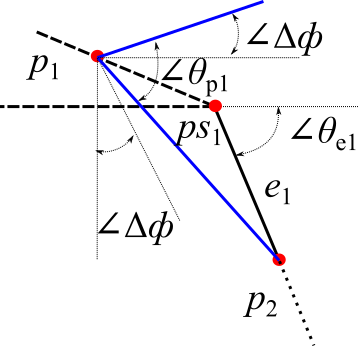
\includegraphics[height=1.3in]{figures/proof_1.png}
\end{center}
\caption{ $p_2$ contact $e_1$ first. }
\label{fig:proof_1}
\end{subfigure}
\begin{subfigure}{0.24\textwidth}
\begin{center}
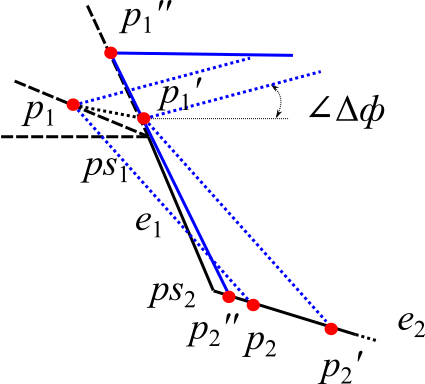
\includegraphics[height=1.3in]{figures/proof_2.png}
\end{center}
\caption{$p_2$ contact $e_2$ first. }
\label{fig:proof_2}
\end{subfigure}
\end{center}
\caption{Induce capture for $\theta_{e1} > \theta_{p1} - \Delta\phi$. }
\label{fig:proof}
\end{figure}
 
\begin{itemize}

\item Figure~\ref{fig:proof_1} shows the case $p_2$ contact $e_1$ first. Easily have the signed distance between $p_1$ and $e_1$ is negative. Denote the start point of $e_1$ as $ps_1$. To ensure the signed distance become non-negative before contacting outside the socket, the moving direction of $p_1$ should no less than $p_1 \to ps_1$.

\begin{enumerate}
\item If $\theta_{e1} \le 2\pi - \Delta\phi$, $p_1$ would move along $ps_1 \to p_2$, which is less than $p_1 \to ps_1$. Contradiction.

\item If $\theta_{e1} > 2\pi - \Delta\phi$, $p_1$ would move along with $\Delta\phi$. Since $\theta_{p1} \le \pi/2$, $\Delta\phi$ is no larger than the direction $p_1 \to ps_1$, thus less than $p_1 \to ps_1$. Contradiction.
\end{enumerate}

Thus, if $\theta_{e1} > \theta_{p1} - \Delta\phi$ and $p_2$ contact $e_1$ first, $p_1$ would contact outside the socket during insertion. 

\item For the case $p_2$ contact $e_2$ first. 

\begin{enumerate}
\item If the signed distance between $p_1$ and $e_1$ is negative, as analyzed above, the direction of $ps_2 \to p_2$ should no less than $p_1 \to ps_1$ to allow $p_1$ captured, where $ps_2$ is the start point of $e_2$.

As shown in Figure~\ref{fig:proof_2}, if $ps_2 \to p_2$ no less than $p_1 \to ps_1$, the signed distance between $p_1$ and $e_1$ can become zero during insertion e.g., $p_1$ and $p_2$ moved to $p_1'$ and $p_2'$, where $p_1'$ is on or above $ps_1$. Then, let $d\theta = 0$, $p_1'$ and $p_2'$ would move to $p_1''$ and $p_2''$. We can see the $p_1''$ must on the extension cord of $e_1$, which means $s < 0 $. Contradiction.

\item If the signed distance between $p_1$ and $e_1$ is not negative. For $\theta_{e2} < \theta_{e1}$, move $p_1$ along $p_2 \to ps_2$ to make signed distance zero. Then do the same with above, we can also get $s < 0 $. For $\theta_{e2} \ge \theta_{e1}$, e.g., collinear and concave cases, which means the singed distance between $p_2$ and $e_1$ is 0 or negative. To make the signed distance between $p_1$ and $e_1$ not negative, the direction of $p_2 \to p_1$ should maintain or increase signed distance to $e_1$, which means $\theta_{e1} \le \theta_{p1} - \Delta\phi$. Contradiction.

\end{enumerate}

If the $p_2$ contact $e_2$ first, to induce the $p_1$ captured, there must be contradictions for $0 \le s \le 1 $ or $\theta_{e1} > \theta_{p1} - \Delta\phi$. 




\end{itemize}


\end{proof}

%\begin{lemma}
%Given a $\Delta x$ and $\Delta\phi$, the initial offset along $x$ axis and orientation for the peg. Denote $\theta_{ei}$ as .... If there is a point of the peg outside the edge of the socket near the entrance ($e_1$), that is, $\Delta x > D - d\cdot \cos\Delta\phi$, $e_1$ needs to be no longer than $\frac{l\cdot\sin(\theta_{e2}-\theta_{p1}-\Delta\phi)}{\sin(\pi - \theta_{e2} + \theta_{e1})}$ to allow the capture of peg with point-edge contacts with socket. 
%\end{lemma}

% comment Weifu: 
% you need to write it like this, and provide a short proof. And you need to provide the computed angle. 
%\begin{proof}

%As $\Delta x > D - d\cdot \cos\Delta\phi$, let $p_1$ be the point outside $e_1$. To ensure the peg be captured, there should be another point contact the surface of the socket before $p_1$ contact outside the socket. Denote the contact inside point as $p_2$, if $p_1$ can move into the socket with the moving of $p_2$ during insertion, the peg is captured.

%Denote $e_i'$ as the parallel line of $e_i$ though the start point of $e_1$. Easily see that, the moving direction of $p_2$ is along $e_2$. Therefore $p_1$ should be on or above $e_i'$ to avoid contact outside the socket.

%Translation $p_2$ to the end point of $e_1$, we can get minimum length of $e_1$ to make $p_1$ on $e_i'$ as shown in Figure~\ref{fig:proof}. That is $\frac{l\cdot\sin(\theta_{e2}-\theta_{p1}-\Delta\phi)}{\sin(\pi - \theta_{e2} + \theta_{e1})}$.

%\end{proof}

Based on the above Lemma, the entrance of the socket needs to be gentle to induce capture, i.e. correcting the displacement along $x$ axis for the peg, before aligning the orientation. In initialization, as the point of the peg defined on the edge of the socket by $s$, if $ \theta_{e1} < \theta_{p1} $, the signed distance between $p_2$ and $e_1$ must be negative. However, if the socket were to be of convex shape, the signed distance between all points of the peg and all edges of the socket should be non-negative.  Therefore, for the convex socket, we must have $ \theta_{e1} \ge \theta_{p1} $, then $ \theta_{e1} > \theta_{p1} - \Delta\phi$ for $\Delta\phi > 0$. It means for the convex socket, we can never induce the peg captured as long as there is a point of the peg outside the socket with $\forall \Delta\phi > 0$. Concave shape sockets, therefore, is much more suitable for insertion. Which means we can actually cut down the loop for $m$, only considering cases where $m > 4$. 

% \subsection{Different number of edges and points}

% The joint can be classified into two main types with respect to the geometry of the socket, e.g., convex and concave. Because the peg is defined by the points which are denoted by $t$ and $\epsilon$, and the edges that connect the points can be variable, we ignore the geometry of the peg. 

% However, there is an important defect for the convex joint: 
% Given the transition error $d x$ and the rotation angle $d \theta$, to simplify, both $d\theta$ and $dx$ are defined as the first time the point of the peg contact inside or outside the socket. Denote the distance between the first point and the last point of the socket and of the peg as $2L$ and $2l$, respectively. Without considering the error $\epsilon$ for the socket, if $ d x > L - l\cos{d\theta}$ and $d \theta > 0$, the peg can not be captured.

% Proof: Denote the angle between the first edge and the last edge of the socket (without the cover edge) as $2 \theta_1$. Denote the angle between the line connecting the first two points of the peg and the line connecting the last two points of the peg as $2 \theta_2$. For the convex joint, we can easily obtain $ \theta_1 < \theta_2$. With $d \theta > 0$, we have $ \theta_1 < \theta_2 + d \theta$.

% As $ d x > L - l\cos{d\theta}$ and $ \theta_1 < \theta_2 + d \theta$, there are three cases for the insertion with respect to the first contact situation during insertion.
% \begin{itemize}
% \item The peg contact outside the socket first. According to the definition, the peg is not captured.

% \item The peg contact outside and inside at the same time. According to the definition, the peg is not captured.

% \item The peg contact inside the socket first. Let $p_i$ denote the point of the peg contact on the edge $e_i$. According to $d x > L - l\cos{d\theta}$, there is a point $p_j$ is outside the socket but do not contact. If the $p_j$ can contact outside the socket during further insertion, the peg is not captured. 

% Prove: Let $l_1$ be the extension cord for $e_1$; $l_2$ be the parallel line of $e_i$ through the start point of $e_1$; $l_3$ be the block plane for the socket. In the further insertion, since the edges of the peg can be curve, the start point of the $e_1$ would not contact the edge of the peg. Therefore, the $d\theta$ would not change, and the $p_j$ would move along the direction of $e_i$. There are also three cases.
% \begin{enumerate}
% \item The $p_j$ is in the area between the $l_2$ and $l_3$. The $p_j$ would contact $l_3$ during insertion, e.g., not captured.

% \item The $p_j$ is on $l_2$. As shown in Figure~\ref{fig:proof},  $p_i$ and $p_j$ would move to $p_i'$ and $p_j'$ during insertion, where $p_j'$ is the start point of the $e_1$. Consider the points of the peg is defined on the edges of the socket by $t$, we can keep the distance between $p_i'$ and $p_j'$ and move the points on the edge to change $d\theta$. Let $d\theta = 0$, $p_i'$ and $p_j'$ would move to $p_i''$ and $p_j''$. We can get that the $p_i''$ is on $l_1$, which means in initialization, $t(i, 1) < 0$. Therefore this case is impossible.

% \item The $p_j$ is in the area between the $l_1$ and $l_2$. The $p_j$ would on $l_1$ during insertion. Similarly, we can get $t(i, 1) < 0$. This case is also impossible.

% \end{enumerate}

% Therefore, the peg contact inside the socket first can not be captured. 

% \end{itemize}

% Above all, for the convex joint, the peg can not be captured, as $ d x > L - l\cos{d\theta}$ and $d \theta > 0$.  Consider optimizing stability would make $l \to L$ and there is a bound for $ d \theta $, the choice of $ d x $ would be very narrow. Therefore, the convex joint is not a good design.

% For the concave joint, we have compared the 5-5 joint and the 4-5 joint. The result shows as follows.
In the case of $m=5$, we find the difference of the possible rotation before and after the optimization for the design, and see a big improvement for the possible rotation, in radian. 

\begin{table}[h!]
  \begin{center}
    \caption{The possible rotations for the joints with $m=5$.}
    \label{tab:table1}
    \begin{tabular}{|c | c | c|}
    \hline
      \textbf{$n-m$ } & \textbf{Max rotation} & \textbf{Max rotation}\\
      \hline
      4-5 joint & 0.1764 & 0.0383\\
      \hline
      5-5 joint & 0.1878 & 0.0372\\
      \hline
    \end{tabular}
  \end{center}
\end{table}


As shown in Table~\ref{tab:table1}, the stability of both joints has been increased after optimizing. However, the difference of stability between the two optimized joints are very small. 

\begin{figure}
\begin{center}
\begin{subfigure}[t]{0.24\textwidth}
\begin{center}
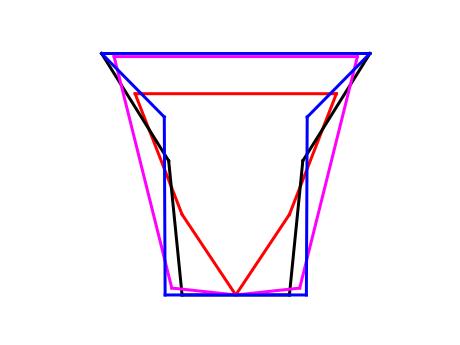
\includegraphics[height=1.3in]{figures/best_5_5_joint.png}
\end{center}
\caption{The initial design (blue and black) and optimized design (red and brown) for the 5-5 joint. }
\label{fig:best_5_5_joint}
\end{subfigure}
\begin{subfigure}[t]{0.24\textwidth}
\begin{center}
\includegraphics[height=1.3in]{figures/best_4_5_joint.png}
\end{center}
\caption{The initial design (blue and black) and optimized design (red and brown) for the 4-5 joint. }
\label{fig:best_4_5_joint}
\end{subfigure}
\caption{The initial design and optimized design for two joints. }
\label{fig:best_joint}
\end{center}
\end{figure}

\section{Conclusion and future work}

In this paper, we have analyzed the ideal peg and socket joint in 2-D plane with respect to the insertion and stability. To analyze the constraint for insertion and the gradient of the stability, we have discretized the insertion process and the "rocking" process for the peg in the socket. Besides, we have proved the concave joint is better than convex joint with respect to capture. The designed algorithm can optimize and compare the peg and socket joint so as to get best peg and socket joint design. In the future, we would extend the 2-D joint design to 3-D, then explore the assembling for the best joint block by the manipulator. 

\renewcommand*{\bibfont}{\small}
\printbibliography

\end{document}
